% vim: set textwidth=78 autoindent:

\subsection{Complemento convertidor Dxf2Shp}

% when the revision of a section has been finalized, 
% comment out the following line:
%\updatedisclaimer

El complemento convertidor dxf2shape puede ser usado para convertir datos vectoriales de DXF al formato Shapefile. Esto requiere que los siguientes parámetros sean especificados antes de la ejecución:

\begin{itemize}
\item \textbf{Archivo DXF de entrada}: Capture la ruta al archivo DXF a ser convertido
\item \textbf{Archivo Shp de salida}: Capture el nombre deseado para el shapefile a ser creado.
\item \textbf{Tipo de archivo de salida}: Especifica el tipo de geometría del shapefile de salida. 
Los tipos actualmente soportados son polilínea, polígono, y punto.
\item \textbf{Exportar etiquetas de texto}: Cuando esta caja de verificación está activada, un Shapefile de puntos adicional será creado, y la tabla dbf asociada contendrá información acerca los campos "TEXT" encontrados en el archivo dxf, y las cadenas de texto mismas.
\end{itemize}

\begin{figure}[ht]
   \begin{center}
   \caption{Complemento convertidor dxf2Shape \nixcaption}\label{fig:dxf2shape_dialog}\smallskip
   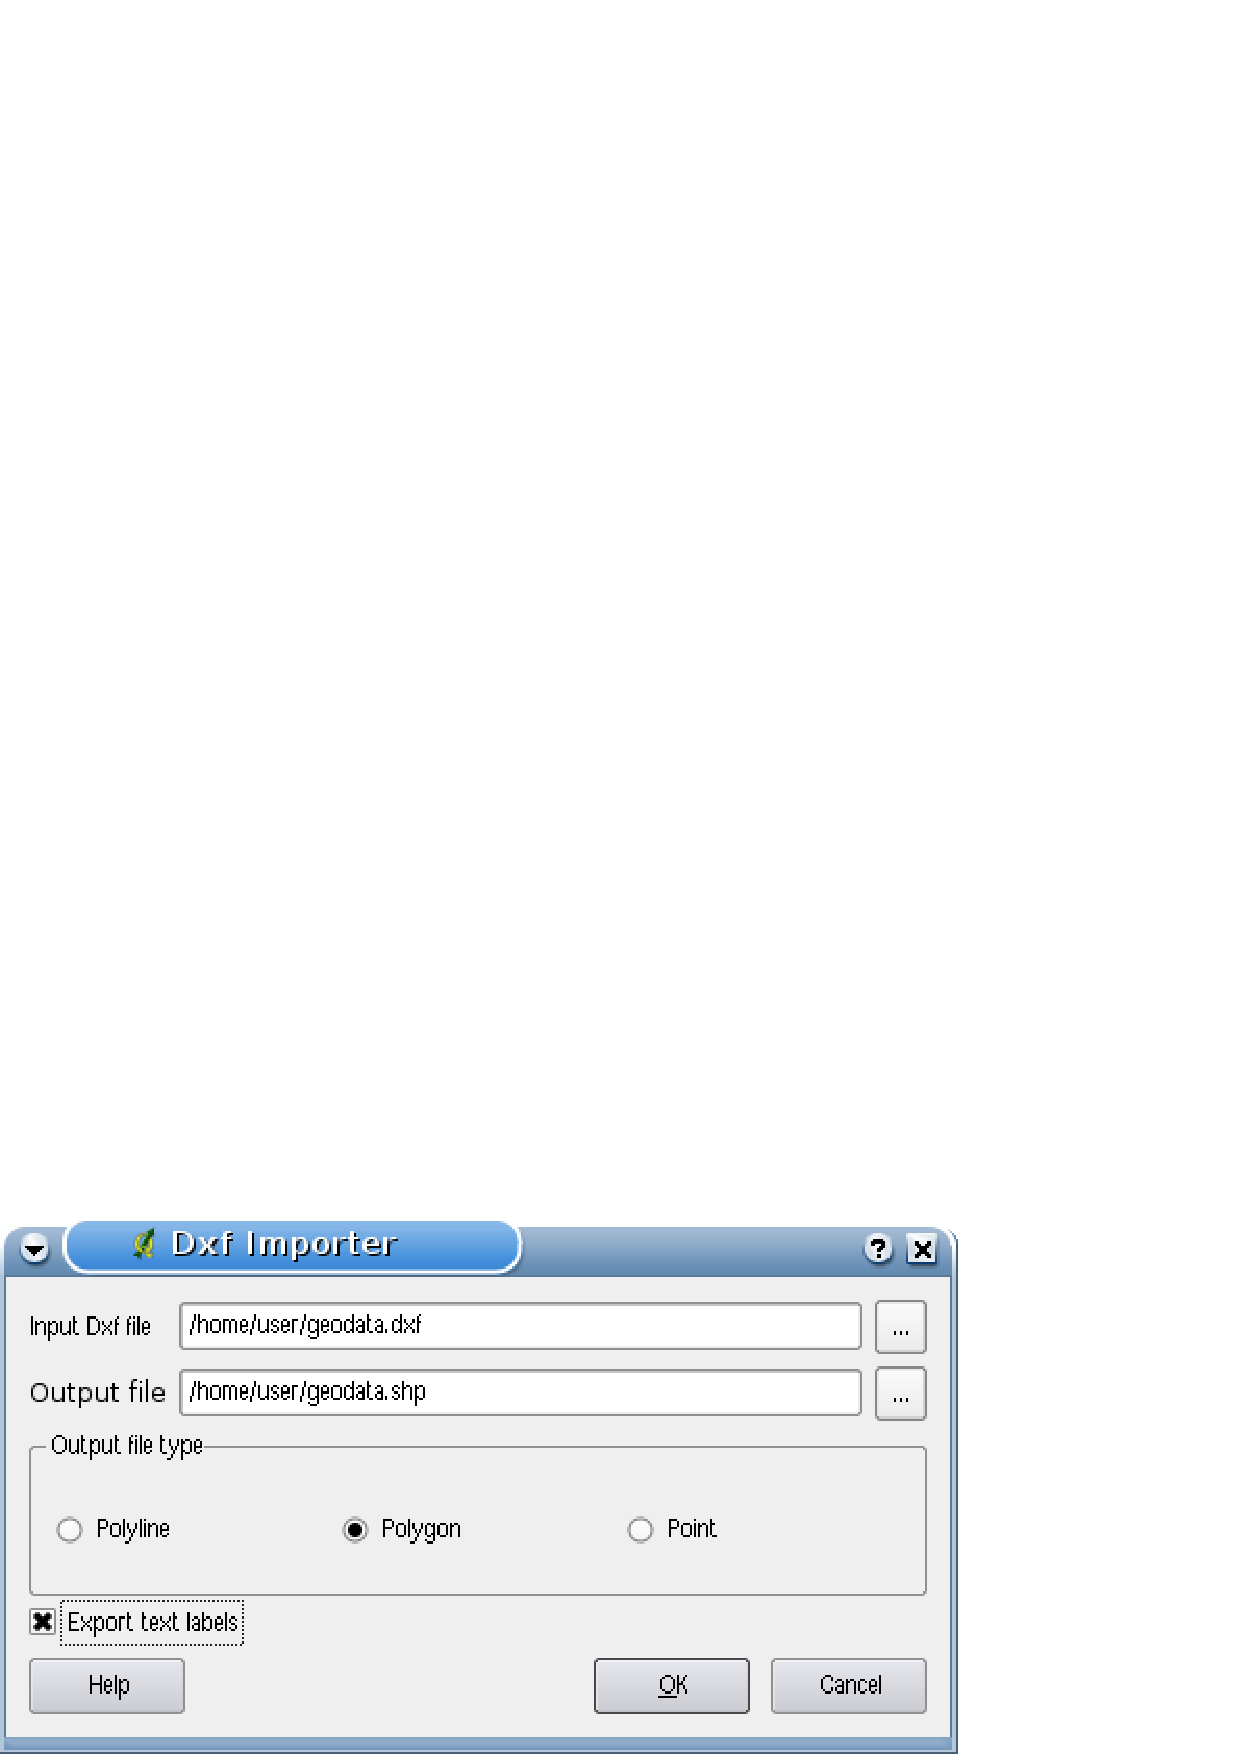
\includegraphics[clip=true, width=12cm]{dxf2shape_dialog}
\end{center}  
\end{figure}

\minisec{Usando el complemento}

\begin{enumerate}
  \item Inicie QGIS, cargue el complemento dxf2Shape en el manejador de complementos (vea la sección 
  \ref{sec:load_core_plugin}) y haga clic en el ícono \toolbtntwo{dxf2shp_converter}{Convertidor dxf2Shape} 
  que aparece en la barra de menús de QGIS. El diálogo del complemento dxf2Shape aparece como se muestra en la figura \ref{fig:dxf2shape_dialog}.
  \item Capture el archivo de entrada DXF, un nombre para el Shapefile de salida y el tipo de Shapefile.
  \item Activar la caja de verificación \checkbox{Exportar etiquetas de texto} si quiere crear una capa de puntos extra con etiquetas.
  \item Clic \button{Ok}. 
\end{enumerate}

\newpage
